\chapter{ကွန်ထရိုးလ် စတိတ်မန့်များ}



\section{Python Arcade Library}
\fEn{Python Arcade} (ဝက်ဘ်ဆိုက် \fCode{https://api.arcade.academy}) ဟာ အရည်အသွေးကောင်းတဲ့ ထိပ်ဆုံး \fEn{Python} ဂိမ်းလိုက်ဘရီတွေထဲက တစ်ခုဖြစ်တယ်။ \fEn{Arcade} အပြင် အသုံးများတဲ့ အခြားတစ်ခုက \fEn{pygame} (ဝက်ဘ်ဆိုက် \fCode{https://www.pygame.org}) ပါ။ ဒီစာအုပ်မှာ \fEn{Arcade} ကို သုံးပါမယ်။ \fEn{Arcade} ပိုကောင်းတယ်လို့ မဆိုလိုပါဘူး။ ဘီဂင်နာတွေအတွက် ပိုသင့်တော်မယ် ယူဆတဲ့အတွက် အသုံးပြုတာပါ။ အောက်ပါအတိုင်း အင်စတောလ်လုပ်နိုင်ပါတယ်
\begin{codetxt}
pip install arcade
\end{codetxt}

\section{Arcade ဖြင့် ပုံဆွဲခြင်း}
ပုံဆွဲလို့ရတဲ့ ဝင်းဒိုးတစ်ခုပေါ်လာအောင်  လိုအပ်တဲ့ အဆင့်တစ်ဆင့်ချင်းကို  အောက်ပါ \fEn{Arcade} ပရိုဂရမ်မှာ တွေ့ရပါမယ်။ ဝင်းဒိုးပေါ်က ရုပ်ပုံတွေကို အန်နီမေးရှင်း \fEn{(animation)} လုပ်တဲ့နည်းကိုလည်း မကြာခင်တွေ့ရမှာပါ။ ပရိုဂရမ် \fEn{run} ရင်
ပုံ (\fRefNo{\ref{fig:ch07starter}})
%
\begin{py}
import arcade

arcade.open_window(300, 200, "Arcade Starter")
arcade.set_viewport(left=0, right=300, top=0, bottom=200)

# Set the background color
arcade.set_background_color(arcade.color.PINK_PEARL)

# Get ready to draw
arcade.start_render()

# Finish drawing
arcade.finish_render()

# Keep the window up until someone closes it.
arcade.run()
\end{py}
%

\begin{figure}[tb!]
\begin{tikzpicture}
    \node[anchor=south west,inner sep=0] (image) at (0,0)
        {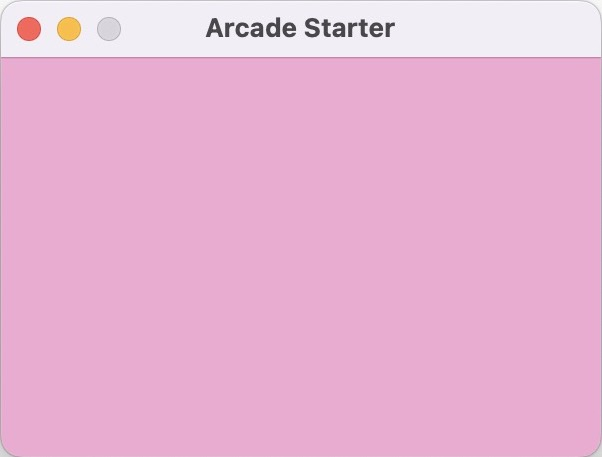
\includegraphics[width=.4\linewidth]{images/ch07/starter.jpg}};
    \drawshadow{image}
\end{tikzpicture}
\caption{}
\label{fig:ch07starter}
\end{figure}

အပေါ်ဆုံးက \fCode{arcade} လိုက်ဘရီ အင်ပို့လုပ်ထားတာပါ။ ရှေ့ပိုင်းမှာသုံးတဲ့ \fCode{from ... import ...} နဲ့ ကွာခြားတာက အခုနည်းနဲ့ အင်ပို့လုပ်ထားရင် လိုက်ဘရီမှာ ပါတဲ့ အစိတ်အပိုင်းတွေကို ဒေါ့ထ်အမှတ်အသားနဲ့ အသုံးပြုရပါမယ်။ ဥပမာ \fCode{open\_window} ဖန်ရှင်ကို
\begin{codetxt}
arcade.open_window(ß\fEnEmp{arguments}ß)
\end{codetxt} 
လိုက်ဘရီ နံမည်နောက်မှာ \fEn{(}\fCodeBf{.}\fEn{)} အမှတ်အသား ခံပြီး ခေါ်ရမှာပါ။ ဒီဖန်ရှင်မှာ လိုချင်တဲ့ဝင်းဒိုး အကျယ်၊ အမြင့်၊ တိုက်တယ်လ်စာသား ထည့်ပေးထားတယ်။ 

အောက်ပါ \fCode{set\_viewport} ဖန်ရှင်ကတော့ ဝင်းဒိုး ကိုဩဒိနိတ်စစ်စတမ် \fEn{origin} အမှတ်နဲ့  $x, y$ ဒါရိုက်ရှင် သတ်မှတ်ပေးတာပါ။
%
\begin{py}
arcade.set_viewport(left=0, right=300, top=0, bottom=200)
\end{py}
%
ဝင်းဒိုး ဘယ်ဘက်စွန်း $x$  ကိုဩဒိနိတ်ကို $0$ နဲ့ ညာဘက်စွန်းကို $300$ သတ်မှတ်ပြီး အပေါ်ဘက်စွန်း (တိုက်တယ်လ်ဘားမပါ) $y$ ကိုဩဒိနိတ်ကို $0$ နဲ့ အောက်ဘက်စွန်းကို $200$ သတ်မှတ်ထားပါတယ်။ တစ်နည်းအား\allowbreak ဖြင့် ဝင်းဒိုးရဲ့ ဘယ်ဘက်အပေါ်ထောင့်စွန်းကို \fEn{origin} အမှတ် $(0,0)$ အဖြစ် သတ်မှတ်တာပါ။ ဘယ်ဘက်ကို သွားရင် $x$ တန်ဖိုး တိုးသွားပြီး အောက်ဘက်ကို ဆင်းရင် $y$ တန်ဖိုး တိုးသွားမှာဖြစ်တယ်။ ကိုယ်တိုင် အခုလို မသတ်မှတ်ပေးဘဲ  အရှိအတိုင်းဆိုရင် ‘အောက်ခြေ’ ဘယ်ဘက်စွန်းကို \fEn{origin} အမှတ် $(0,0)$ အဖြစ် \fEn{Arcade} က သတ်မှတ်တယ်။ \fCode{set\_viewport} ကို ဒီလိုခေါ်ထားတာနဲ့ တူမယ်
%
\begin{py}
arcade.set_viewport(left=0, right=300, top=200, bottom=0)
\end{py}
%
ဒီလိုနည်းက အခြား ဂိမ်း လိုက်ဘရီတွေနဲ့ မတူဘဲဖြစ်နေတဲ့အတွက်  လိုက်ဘရီပြောင်းသုံးရင် အခက်အခဲရှိနိုင်တယ်။ ဒါကြောင့် အခြားလိုက်ဘရီတွေ နည်းတူဖြစ်အောင် အရှိအတိုင်းမသုံးဘဲ ကိုယ်ပိုင် သတ်မှတ်ပေးရတာပါ။

အောက်ပါ ဖန်ရှင်ကတော့ ဝင်းဒိုးရဲ့ နောက်ခံရောင် သတ်မှတ်တာပါ။ လိုက်ဘရီရဲ့ \fCode{color} မော်ဒျူး \fEn{(\textit{module})} မှာ အရောင်တန်ဖိုးတွေ အဆင်သင့် သတ်မှတ်ပေးထားတယ်။ (မော်ဒျူးဆိုတာ လိုက်ဘရီရဲ့ အစိတ်အပိုင်းတစ်ခုလို့ အကြမ်းဖျဉ်း ယူဆနိုင်တယ်)။ 
%
\begin{py}
arcade.set_background_color(arcade.color.PINK_PEARL)
\end{py}
%
အခုလို အင်ပို့လုပ်ထားရင် အရောင်တွေ သုံးရတာ ပိုအဆင်ပြေတယ်
%
\begin{py}
import arcade
from arcade.color import *
ß$\ldots$ß
arcade.set_background_color(PINK_PEARL)
\end{py}
%
\fCode{PINK\_PEARL}\fEn{,} \fCode{RED} စသည်ဖြင့် အရောင်နံမည် တမ်းရေးလို့ရတယ်။ ရှေ့မှာ \fCode{arcade.color.} ထည့်ဖို့  မလိုတော့ဘူး။

ပုံဆွဲဖို့ အဆင်သင့်ဖြစ်အောင် \fCode{start\_render} ခေါ်ပေးရပါမယ်။ ပြီးရင်လည်း \fCode{finish\_render} ခေါ်ဖို့လိုတယ်။ ၎င်းတို့နှစ်ခုကြားမှာ \fEn{Arcade} နဲ့ ပုံဆွဲတဲ့ ဖန်ရှင်တွေကို  ခေါ်ရမှာပါ။
%
\begin{py}
arcade.start_render()
# call drawing functions here
ß$\ldots$ß
ß$\ldots$ß
arcade.finish_render()
\end{py}
%
\betweenminted{\medskipamount}
%
\begin{py}
arcade.run()
\end{py}
%
ဝင်းဒိုးကို မပိတ်မချင်း ပေါ်နေအောင် \fCode{run} ဖန်ရှင် ခေါ်ပေးရတာပါ။ မခေါ်ထားဘဲ ပရိုဂရမ်ကို \fEn{run} ရင် ဝင်းဒိုးပွင့်လာပြီး ဖျတ်ခနဲ ပြန်ပိတ်သွားမှာပါ။ မကျန်ခဲ့ဖို့ သတိပြုရပါမယ်။

\fEn{Arcade} မှာ ပါတဲ့ အခြေခံ ပုံဆွဲဖန်ရှင် တချို့ကို ဆက်ကြည့်ရအောင်။ ထောင့်မှန်စတုဂံဆွဲတဲ့ ဖန်ရှင်တွေထဲက နှစ်ခု သုံးပြထားတယ်။ နှစ်ခုလုံးက  ထောင့်မှန်စတုဂံရဲ့ ဘယ်ဘက်အပေါ်ထောင့်စွန်းနဲ့ တည်နေရာကို သတ်မှတ်ပြီး အရွယ်အစားကို အကျယ်၊ အမြင့်နဲ့ သတ်မှတ်ပေးရတာပါ။  \fCode{draw\_xywh\_rec\allowbreak tangle\_filled} က အတွင်းပိုင်း အရောင်နဲ့ ဆွဲပေးတယ်။ အနားတွေကိုပဲ ဆွဲချင်ရင် \fCode{draw\_xywh\_rec\allowbreak tangle\_outline} ဖန်ရှင်သုံးရပါမယ်။
%
\begin{py}
import arcade
from arcade.color import *

arcade.open_window(300, 200, "Drawing Example")
arcade.set_viewport(0,300, 200, 0)

arcade.set_background_color(PINK_PEARL)
arcade.start_render()
# start drawing
arcade.draw_xywh_rectangle_filled(5,5,200, 50,BABY_BLUE)
arcade.draw_xywh_rectangle_outline(5,5,200, 50,BLACK)

arcade.draw_xywh_rectangle_filled(5,55,200, 50,PALE_VIOLET_RED)
arcade.draw_xywh_rectangle_outline(5,55,200, 50,BLACK)
#finish drawing
arcade.finish_render()
arcade.run()
\end{py}
%
ဒါကို \fEn{run} လိုက်ရင် ပုံ (\fRefNo{\ref{fig:ch07rects}}) မှာလို တွေ့ရမှာပါ။ အနက်ရောင် အနားသတ်နဲ့ အပြာရောင်ဖြည့်ထားတဲ့ အပေါ်ပုံကို ဒီနှစ်ခုနဲ့ 
%
\begin{py}
arcade.draw_xywh_rectangle_filled(5,5,200, 50,BABY_BLUE)
arcade.draw_xywh_rectangle_outline(5,5,200, 50,BLACK)
\end{py}
%
ဆွဲထားတာပါ။ ပါရာမီတာတွေက $x, y, width, height, color$ အစဉ်အတိုင်းဖြစ်တယ်။ $x = 5$ ဖြစ်လို့ ဘယ်ဘက် နည်းနည်းရောက်နေတာပါ။ $y = 5$ ဖြစ်လို့ အောက်ဘက် နည်းနည်းရောက်နေတာပါ။ သုညထားပြီး စမ်းကြည့်ပါ။ အခြားတန်ဖိုးတွေ ပြောင်းလဲပြီးလည်း စမ်းကြည့်ပါ။ ပိုပြီးသဘောပေါက် လာပါလိမ့်မယ်။ အောက်ဘက် ထောင့်မှန်စတုဂံကို ဒီနှစ်ခုနဲ့
%
\begin{py}
arcade.draw_xywh_rectangle_filled(5,55,200, 50,PALE_VIOLET_RED)
arcade.draw_xywh_rectangle_outline(5,55,200, 50,BLACK)
\end{py}
%
ဆွဲထားတာပါ။ ဘယ်ဘက်ခွာထားတဲ့ အကွာအဝေး အပေါ်နဲ့ တူပါမယ် $(x = 5)$။ အပေါ်ပုံရဲ့ အောက်ခြေအနားနဲ့ ကပ်နေအောင် $y = 5 + 50 = 55$ ထားရပါမယ်။



%
\begin{py}
def draw_xywh_rectangle_filled(bottom_left_x: float,
                               bottom_left_y: float,
                               width: float,
                               height: float,
                               color: tuple[int, int, int] 
                                   | list[int] 
                                   | tuple[int, int, int, int]) -> None

def draw_xywh_rectangle_outline(bottom_left_x: float,
                                bottom_left_y: float,
                                width: float,
                                height: float,
                                color: tuple[int, int, int] 
                                    | list[int] 
                                    | tuple[int, int, int, int],
                                border_width: float = 1) -> None
\end{py}
%

\fEn{Arcade} ဝင်းဒိုး \fEn{origin} က သူ့နဂိုအတိုင်းဆိုရင် အောက်ခြေဘယ်ဘက်စွန်းလို့ ရှေ့မှာ ပြောခဲ့ပါတယ်။ \fCode{set\_viewport} နဲ့ အပေါ်ဘယ်ဘက်စွန်းကို \fEn{origin} အဖြစ်ပြောင်းလဲ သတ်မှတ်ထားတယ်။ ဒီ့အတွက်ကြောင့် အထက်အောက် ပြောင်းပြန်ဖြစ်သွားပါတယ်။ 





\begin{figure}[tb!]
\begin{tikzpicture}
    \node[anchor=south west,inner sep=0] (image) at (0,0)
        {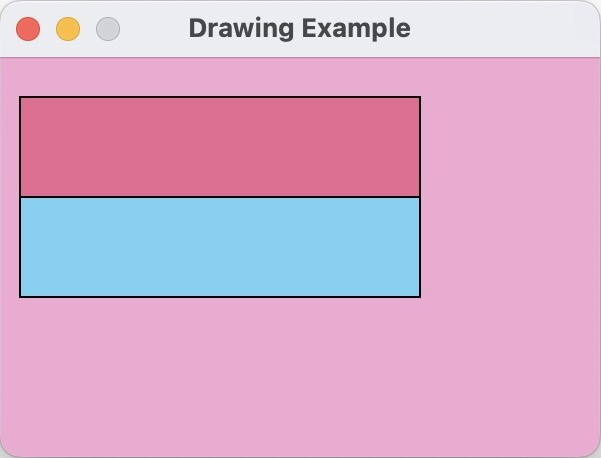
\includegraphics[width=.4\linewidth,trim={0mm 0mm 0mm 0.03mm}]{images/ch07/rects.jpg}};
    \drawshadow{image}
\end{tikzpicture}
\caption{}
\label{fig:ch07rects}
\end{figure}

%
\begin{py}
import arcade
from arcade.color import *

WIN_WIDTH = 600
BOARD_SIZE = 400
WIN_HEIGHT = 420
arcade.open_window(WIN_WIDTH, WIN_HEIGHT, "Arcade Checkerboard")
arcade.set_viewport(left=0,
                    right=WIN_WIDTH,
                    top=0,
                    bottom=WIN_HEIGHT)
arcade.set_background_color(WHITE_SMOKE)
arcade.start_render()

COLS = 8
ROWS = 8
SQ_SIZE = BOARD_SIZE / ROWS
X_LFT = (WIN_WIDTH - BOARD_SIZE) / 2
Y_TOP = (WIN_HEIGHT - BOARD_SIZE) / 2 + 1

for i in range(ROWS):
    for j in range(COLS):
        x = X_LFT + SQ_SIZE * i
        y = Y_TOP + SQ_SIZE * j
        if (i + j) % 2 == 0:
            arcade.draw_xywh_rectangle_filled(x,
                                              y,
                                              SQ_SIZE,
                                              SQ_SIZE,
                                              WOOD_BROWN)
        else:
            arcade.draw_xywh_rectangle_filled(x,
                                              y,
                                              SQ_SIZE,
                                              SQ_SIZE,
                                              BLACK)
        arcade.draw_xywh_rectangle_outline(x,
                                           y,
                                           SQ_SIZE,
                                           SQ_SIZE,
                                           BLACK)

arcade.finish_render()
arcade.run()

\end{py}
%

\begin{figure}[tb!]
\begin{tikzpicture}
    \node[anchor=south west,inner sep=0] (image) at (0,0)
        {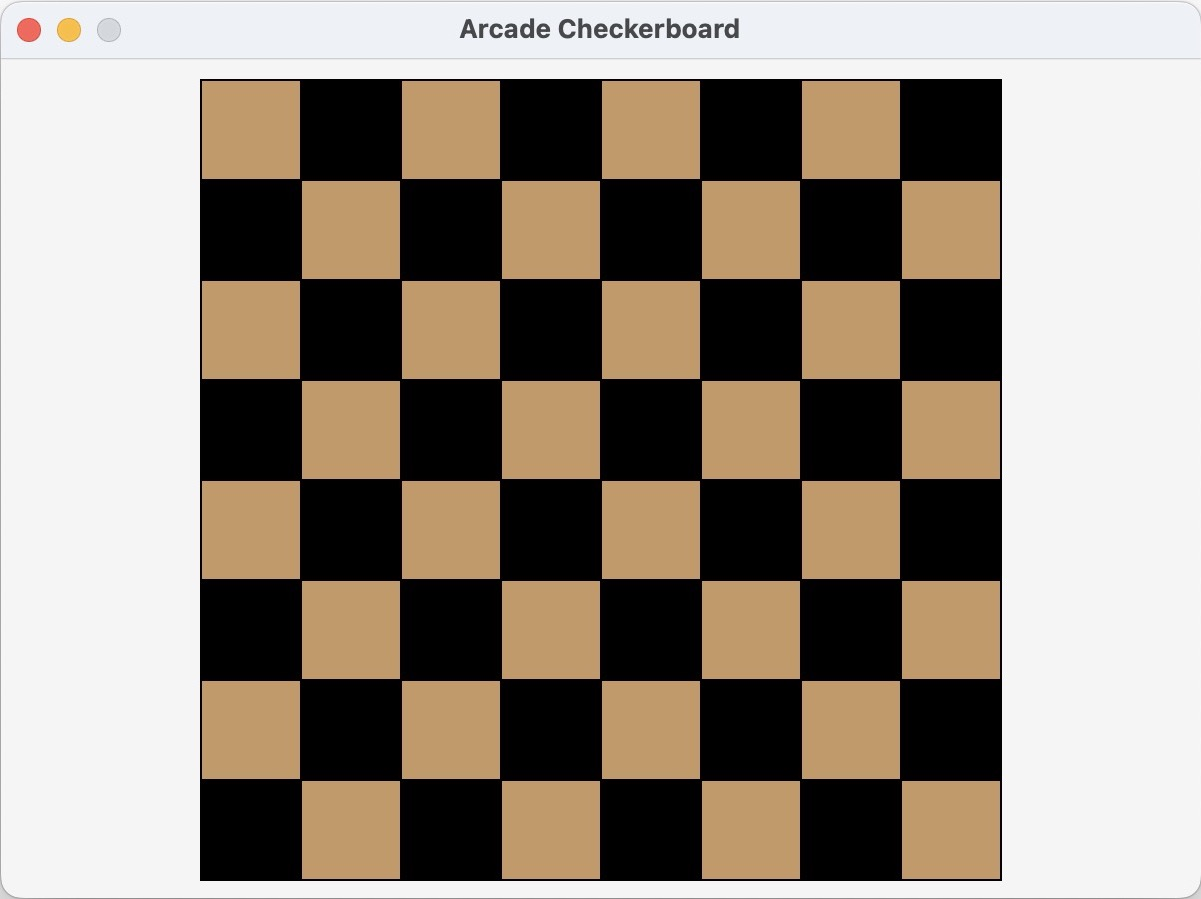
\includegraphics[width=.85\linewidth]{images/ch07/checkerboard.jpg}};
    \drawshadow{image}
\end{tikzpicture}
\caption{}
\label{fig:meet_karel_1}
\end{figure}